\documentclass[11pt,letterpaper]{article}
\usepackage[lmargin=1in,rmargin=1in,tmargin=1in,bmargin=1in]{geometry}
\usepackage{../style/homework}
\usepackage{../style/commands}
\setbool{quotetype}{true} % True: Side; False: Under
\setbool{hideans}{false} % Student: True; Instructor: False

% -------------------
% Content
% -------------------
\begin{document}

\homework{1: Due 09/11}{I'm fine. It's just that life is pointless and nothing matters and I'm always tired.}{Andy Dwyer, Parks and Recreation}

% Problem 4
\problem{10} Complete the following:
	\begin{enumerate}[(a)]
	\item List all the divisors of 80.
	\item List all the nonnegative multiples of 15 less than 180. 
	\end{enumerate} \pspace

\sol 
\begin{enumerate}[(a)]
\item We know that 1 and 80 are divisors (factors) of 80---the improper divisors. Because 80 is even, we know it is divisible by 2. Because the last two digits of 80 are divisible by 4, we know 4 is a divisor of 80. Furthermore, because 80 ends in a 0, it is a multiple of 5 and 10; hence, 5 and 10 are divisors of 80. But then the divisors of 80 are\dots
	\[
	\text{divisors of 80}= \{ 1, 2, 4, 5, 8, 10, 16, 20, 40, 80 \}
	\] \pspace

\item The nonnegative multiples of 15 will be integers of the form $15k$, where $k \geq 0$ is an integer. But then we have\dots \par
	\begin{table}[h]
	\centering
	\begin{tabular}{r|cccccccccccc}
	$k$ & 0 & 1 & 2 & 3 & 4 & 5 & 6 & 7 & 8 & 9 & 10 & 11 \\ \hline
	$15k$ & 0 & 15 & 30 & 45 & 60 & 75 & 90 & 105 & 120 & 135 & 150 & 165
	\end{tabular}
	\end{table} \par
\end{enumerate}



\newpage



% Problem 2
\problem{10} Showing all your work, find the prime factorizations of the following:
	\begin{enumerate}[(a)]
	\item $40$
	\item $90$
	\item $97$
	\item $99$
	\item $228$
	\end{enumerate} \pspace

\sol 
\begin{enumerate}[(a)]
\item $40= 2^3 \cdot 5$
	\[
	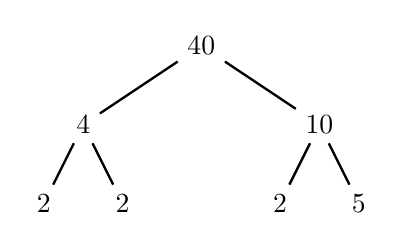
\begin{tikzpicture}
	\node at (0,0) (n) {40};
	\node at (-1.5,-1) (a) {4};
	\node at (1.5,-1) (b) {10};
	\node at (-2,-2) (c) {2};
	\node at (-1,-2) (d) {2};
	\node at (1,-2) (e) {2};
	\node at (2,-2) (f) {5};
	
	\draw[line width=0.03cm] (n) -- (a);
	\draw[line width=0.03cm] (n) -- (b);
	\draw[line width=0.03cm] (a) -- (c);
	\draw[line width=0.03cm] (a) -- (d);
	\draw[line width=0.03cm] (b) -- (e);
	\draw[line width=0.03cm] (b) -- (f);
	\end{tikzpicture}
	\]

\item $90= 2 \cdot 3^2 \cdot 5$
	\[
	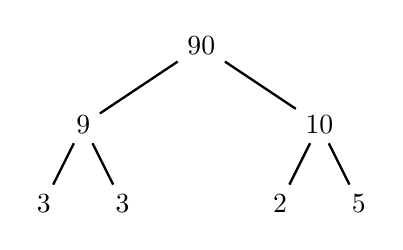
\begin{tikzpicture}
	\node at (0,0) (n) {90};
	\node at (-1.5,-1) (a) {9};
	\node at (1.5,-1) (b) {10};
	\node at (-2,-2) (c) {3};
	\node at (-1,-2) (d) {3};
	\node at (1,-2) (e) {2};
	\node at (2,-2) (f) {5};
	
	\draw[line width=0.03cm] (n) -- (a);
	\draw[line width=0.03cm] (n) -- (b);
	\draw[line width=0.03cm] (a) -- (c);
	\draw[line width=0.03cm] (a) -- (d);
	\draw[line width=0.03cm] (b) -- (e);
	\draw[line width=0.03cm] (b) -- (f);
	\end{tikzpicture}
	\]

\item Observe that $\sqrt{97} \approx 9.85$. If $97$ is composite, then it has a (prime) factor between 2 and 9. We know that 2 does not divide 97 because it is not even. We know also that 3 and 9 do not divide 97 because $9 + 7= 16$ is not divisible by 3 or 9, respectively. We know that 97 is not divisible by 5 because it does not end in 5 or 0. But then 97 does not have a prime factor between 2 and 9. Therefore, 97 is prime, so that the prime factorization is itself. 

\item $99= 3^2 \cdot 11$
	\[
	\begin{tikzpicture}
	\node at (0,0) (n) {99};
	\node at (-1.5,-1) (a) {9};
	\node at (1.5,-1) (b) {11};
	\node at (-2,-2) (c) {3};
	\node at (-1,-2) (d) {3};
	
	\draw[line width=0.03cm] (n) -- (a);
	\draw[line width=0.03cm] (n) -- (b);
	\draw[line width=0.03cm] (a) -- (c);
	\draw[line width=0.03cm] (a) -- (d);
	\end{tikzpicture}
	\]

\item $228= 2^2 \cdot 3 \cdot 19$
	\[
	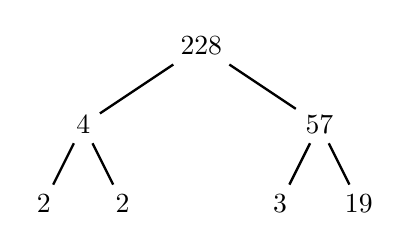
\begin{tikzpicture}
	\node at (0,0) (n) {228};
	\node at (-1.5,-1) (a) {4};
	\node at (1.5,-1) (b) {57};
	\node at (-2,-2) (c) {2};
	\node at (-1,-2) (d) {2};
	\node at (1,-2) (e) {3};
	\node at (2,-2) (f) {19};
	
	\draw[line width=0.03cm] (n) -- (a);
	\draw[line width=0.03cm] (n) -- (b);
	\draw[line width=0.03cm] (a) -- (c);
	\draw[line width=0.03cm] (a) -- (d);
	\draw[line width=0.03cm] (b) -- (e);
	\draw[line width=0.03cm] (b) -- (f);
	\end{tikzpicture}
	\]
\end{enumerate}



\newpage



% Problem 3
\problem{10} Without using a calculator, answer the following:
	\begin{enumerate}[(a)]
	\item Does 2 divide 8455? Explain.
	\item Does 3 divide 19436? Explain.
	\item Does 4 divide 764136? Explain.
	\item Does 5 divide 99999? Explain.
	\item Does 9 divide 331443? Explain. 
	\end{enumerate} \pspace

\sol 
\begin{enumerate}[(a)]
\item No. We know that 8455 is not even, i.e. it is odd; therefore, 2 cannot divide 8455. \pspace

\item No. We know that the sum of the digits is $1 + 9 + 4 + 3 + 6= 23$, which is not divisible by 3; therefore, 19436 is not divisible by 3. \pspace

\item Yes. Because the last two digits of 764136, i.e. 36, are divisible by 4, we know that 764136 is divisible by 4. \pspace

\item No. We know that 99999 does not end in a 5 or 0; therefore, 99999 is not divisible by 5. \pspace

\item Yes. We know that the sum of the digits is $3 + 3 + 1 + 4 + 4 + 3= 18$, which is divisible by 9; therefore, 331443 is divisible by 9. 
\end{enumerate}



\newpage



% Problem 4
\problem{10} Complete the following:
	\begin{enumerate}[(a)]
	\item List all the prime numbers up to 34.
	\item Compute $\sqrt{1223}$.
	\item Using (a) and (b), explain why 1223 is a prime number. 
	\end{enumerate} \pspace

\sol 
\begin{enumerate}[(a)]
\item The primes up to 34 are 2, 3, 5, 7, 11, 13, 17, 19, 23, 29, and 31. \pspace

\item We have $\sqrt{1223} \approx 34.97$. \pspace

\item Observe that none of 2, 3, 5, 7, 11, 13, 17, 19, 23, 29, and 31 divide 1223 because\dots
	\[
	\begin{aligned}
	\dfrac{1223}{2}&\approx 611.5 &\quad \dfrac{1223}{7}&\approx 174.714 &\quad \dfrac{1223}{17}&\approx 71.9412 &\quad \dfrac{1223}{29}&\approx 42.1724 \\
	\dfrac{1223}{3}&\approx 407.667 & \dfrac{1223}{11}&\approx 111.182 & \dfrac{1223}{19}&\approx 64.3684 & \dfrac{1223}{31}&\approx 39.4516 \\
	\dfrac{1223}{5}&\approx 244.6 & \dfrac{1223}{13}&\approx 94.0769 & \dfrac{1223}{23}&\approx 53.1739
	\end{aligned}
	\]
If 1223 were composite, it would have a (prime) divisor between 2 and 34 (because $\sqrt{1223} \approx 34.97$). But from the work above, we know that 1223 has no prime divisor between 2 and 34. Therefore, it must be that 1223 is not composite, i.e. that 1223 is prime. 
\end{enumerate}



\newpage



% Problem 5
\problem{10} Showing all your work, compute the following:
	\begin{enumerate}[(a)]
	\item $\gcd(15, 33)$
	\item $\lcm(15, 33)$
	\item $\gcd(2^{70} \cdot 3^{40} \cdot 7^{60} \cdot 11^{20},\, 2^{90} \cdot 5^{48} \cdot 7^{50} \cdot 11^{20})$
	\item $\lcm(2^{70} \cdot 3^{40} \cdot 7^{60} \cdot 11^{20},\, 2^{90} \cdot 5^{48} \cdot 7^{50} \cdot 11^{20})$
	\end{enumerate} \pspace

\sol We use the fact that the gcd of a collection of numbers is the product of the smallest possible power of the primes found in their prime factorizations and the lcm is the product of the largest possible power of the primes found in their prime factorizations. 
\begin{enumerate}[(a)]
\item 
	\[
	\gcd(15, 33)= \gcd(3 \cdot 5, 3 \cdot 11)= 3^1 \cdot 5^0 \cdot 11^0= 3
	\] \pspace

\item 
	\[
	\lcm(15, 33)= \lcm(3 \cdot 5, 3 \cdot 11)= 3^1 \cdot 5^1 \cdot 11^1= 165
	\] \pspace

\item 
	\[
	\begin{gathered}
	\gcd(2^{70} \cdot 3^{40} \cdot 7^{60} \cdot 11^{20},\, 2^{90} \cdot 5^{48} \cdot 7^{50} \cdot 11^{20})= 2^{70} \cdot 3^0 \cdot 5^0 \cdot 7^{50} \cdot 11^{20}= \\[0.3cm]
1428418283195996611835613989747765760457683489237595071761327175447378932317894475776
	\end{gathered}
	\] \pspace

\item 
	\[
	\begin{gathered}
	\lcm(2^{70} \cdot 3^{40} \cdot 7^{60} \cdot 11^{20},\, 2^{90} \cdot 5^{48} \cdot 7^{50} \cdot 11^{20})= 2^{90} \cdot 3^{40} \cdot 5^{48} \cdot 7^{60} \cdot 11^{20}= \\ {\scriptstyle 35971927533072582764858436471653678010579745561903104000000000000000000000000000000000000000000000000}
	\end{gathered}
	\] \pspace
\end{enumerate}



\newpage



% Problem 6
\problem{10} Isabella has two large wood strips. One is 70~ft long and the other is 98~ft long. She needs to cut them down into boards. The size of the boards does not matter, so long as they are all of equal size. She has a `template' that will let her cut the wood to specific integer lengths, but it must be reset if you change the length---which is time consuming. To what length should she set the template in order to never have to reset it and cut each strip into pieces of equal length? \pspace

\sol Suppose that she can set the template to cut the wood to an integer length $\ell$. Because she is cutting the pieces of wood into some integer number of pieces, each of length $\ell$, it must be that 70 and 98 are both multiples of $\ell$; that is, $\ell$ is a divisor of both 70 and 98. But then $\ell$ is a common divisor of 70 and 98. We can list the divisors of both 70 and 98:
	\[
	\begin{aligned}
	70&\colon \mathbf{1}, \mathbf{2}, 5, \mathbf{7}, 10, \mathbf{14}, 35, 70 \\
	98&\colon \mathbf{1}, \mathbf{2}, \mathbf{7}, \mathbf{14}, 49, 98
	\end{aligned} 
	\]
The common divisors are 1, 2, 7, and 14. Therefore, the possibilities for $\ell$ are 1, 2, 7, 14, and all are viable choices. \pspace

$\ell= 1$~ft: Choosing $\ell= 1$~ft (the smallest possible divisor) obtains the maximum number of pieces. This splits the 70~ft strip into 70~pieces, the 98~ft board into 98~pieces, for a total of 168~pieces of 1~ft length wood. \pspace

$\ell= 2$~ft: Choosing $\ell= 2$~ft splits the 70~ft strip into 35~pieces and the 98~ft strip into 49~pieces, for a total of 84~pieces of 2~ft length wood. \pspace

$\ell= 7$~ft: Choosing $\ell= 7$~ft splits the 70~ft strip into 10~pieces and the 98~ft strip into 14~pieces, for a total of 24~pieces of 7~ft length wood. \pspace

$\ell= 14$~ft: Choosing $\ell= 14$~ft (the greatest common divisor) obtains the minimum number of pieces. This splits the 70~ft strip into 5~pieces and the 98~ft board into 7~pieces, for a total of 12~pieces of 14~ft length wood. \pspace

We can summarize the data below: \par
	\begin{table}[h]
	\centering
	\begin{tabular}{r||c|c|c|c}
	Guide Setting & 1 & 2 & 7 & 14 \\ \hline
	Number Pieces & 168 & 84 & 24 & 12
	\end{tabular}
	\end{table}


\end{document}